%*************************************
% บทที่ 4
%*************************************
\chapterTitle{4}{ผลการดำเนินงาน}

\hspace*{1.3em}
ในการพัฒนา เว็บแอปพลิเคชันเพื่อการคอนฟิกด้วยวิธี NETCONF ผ่าน LLM ได้จัดทำโครงสร้างและการปรับแต่งระบบให้สอดคล้องกับมาตรฐานที่กำหนด ประกอบด้วยการจัดการอุปกรณ์ การสร้างและปรับใช้การกำหนดค่า การสำรองข้อมูล และการประมวลผลด้วย LLM
\section{ผลการดำเนินงาน}
\hspace*{1.3em}
รายละเอียดการทำงานของโปรแกรมผลการดำเนินงานในการจัดทำโครงงานเว็บแอปพลิเคชันเพื่อการคอนฟิกด้วยวิธี NETCONF ผ่าน LLM มีรายละเอียดดังนี้

\begin{figure}[H]
\centering
\adjustbox{frame, width=1.0\textwidth}{%สร้างกรอบของภาพ
    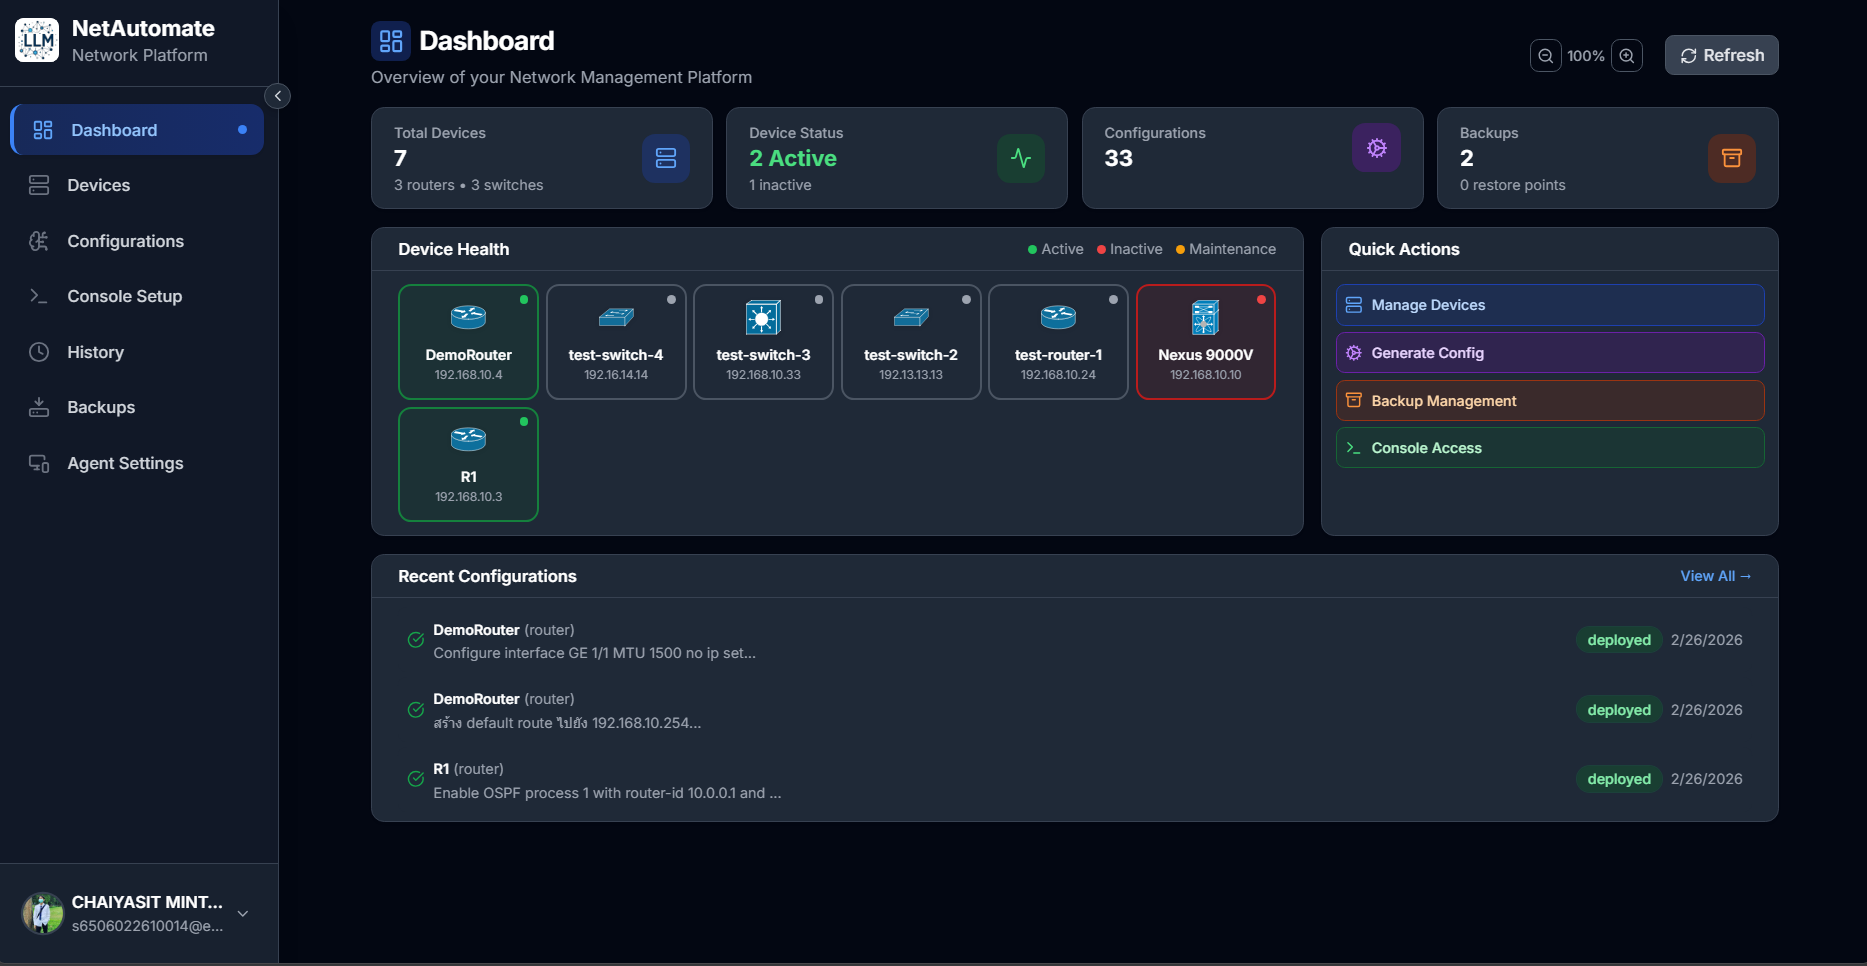
\includegraphics[width=1.0\textwidth]{Image/dashboard-1.png}
}
\caption{\fontSixTeen{หน้าจอ Dashboard}}
\label{fig4:Dashboard}
\end{figure}

\hspace*{1.3em} %ย่อหน้า
จากภาพที่ \ref{fig4:Dashboard} แสดงภาพรวมของระบบ ระบุจำนวนอุปกรณ์ที่เชื่อมต่ออยู่และจำนวน Configurations ที่มีอยู่ในระบบและแสดงรายรายละเอียดของอุปกรณ์ IP Address, Model, Location, Status และรายละเอียดของ Configurations 5 ครั้งล่าสุด


\begin{figure}[H]
\centering
\adjustbox{frame, width=1.0\textwidth}{%สร้างกรอบของภาพ
    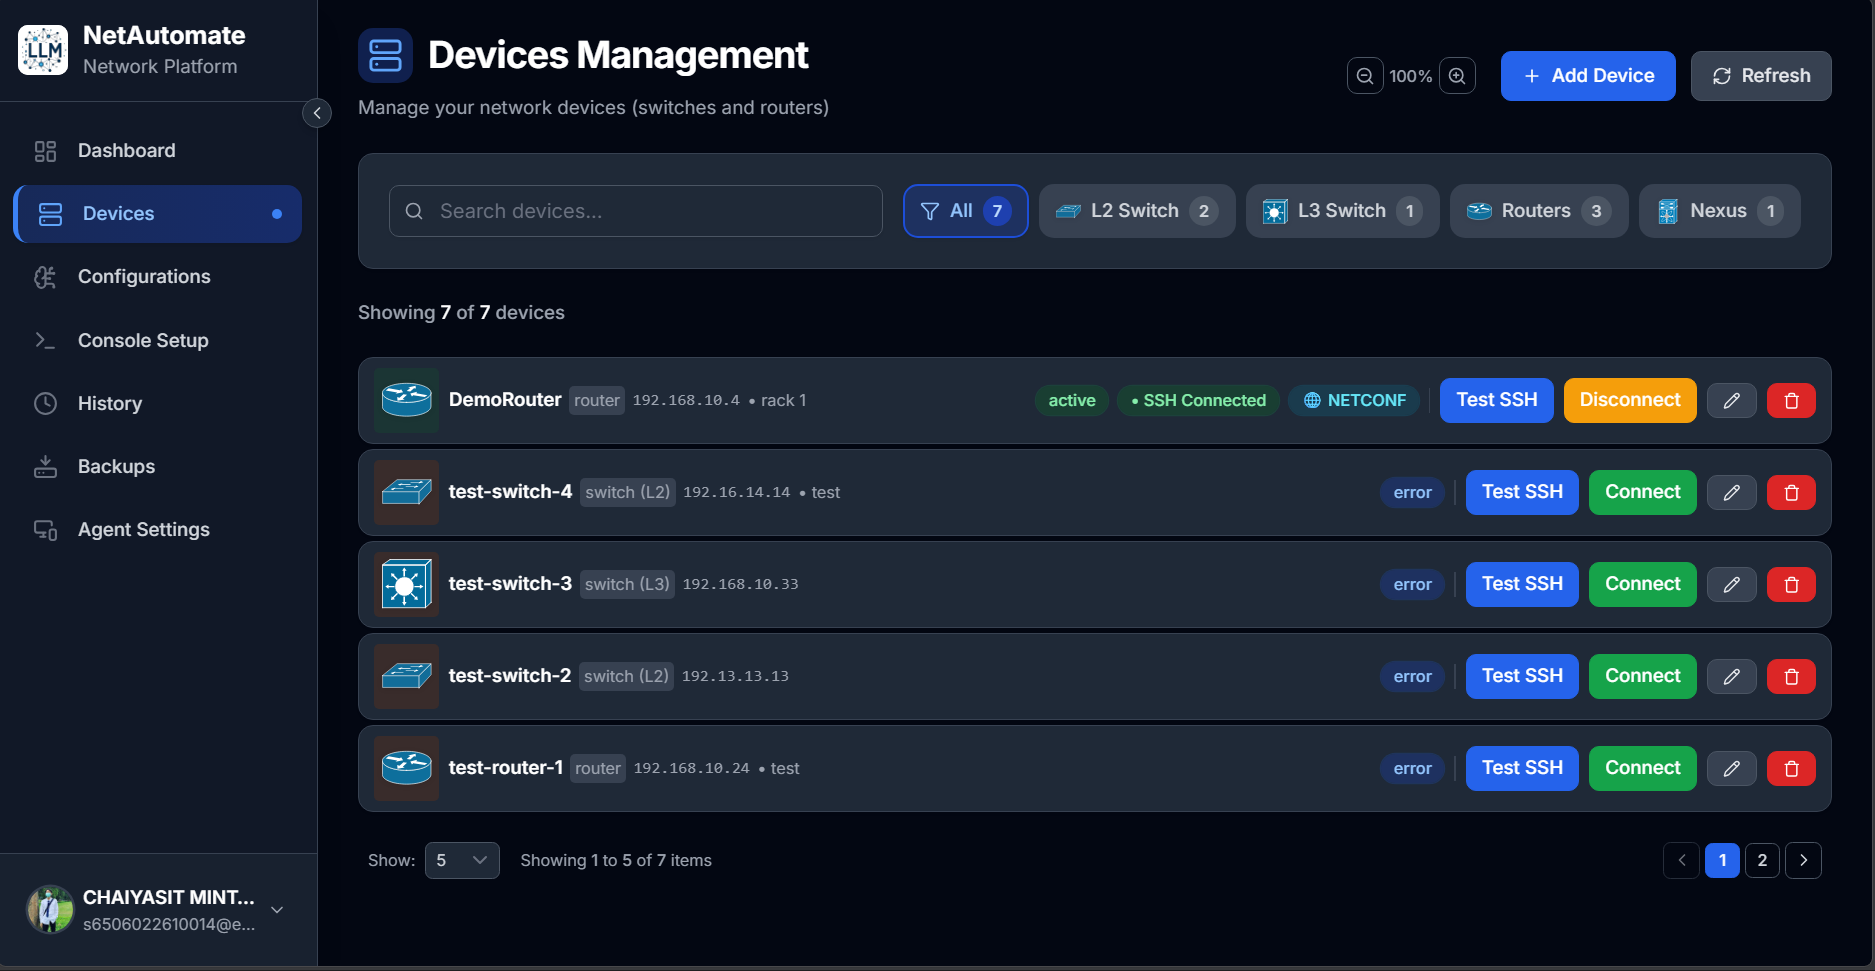
\includegraphics[width=1.0\textwidth]{Image/device-mgmt-1.png}
}
\caption{\fontSixTeen{หน้าจอ Device Management}}
\label{fig4:DeviceManage}
\end{figure}

\hspace*{1.3em} %ย่อหน้า
จากภาพที่ \ref{fig4:DeviceManage} แสดงหน้าจอสำหรับการจัดการอุปกรณ์ในระบบ สำหรับกรอกข้อมูลเริ่มต้นในการเชื่อมต่อกับอุปกรณ์ IP Address, Username, Password, Type ของอุปกรณ์ และ การเสิร์ชหาด้วยฟิลเตอร์

\begin{figure}[H]
\centering
\adjustbox{frame, width=1.0\textwidth}{%สร้างกรอบของภาพ
    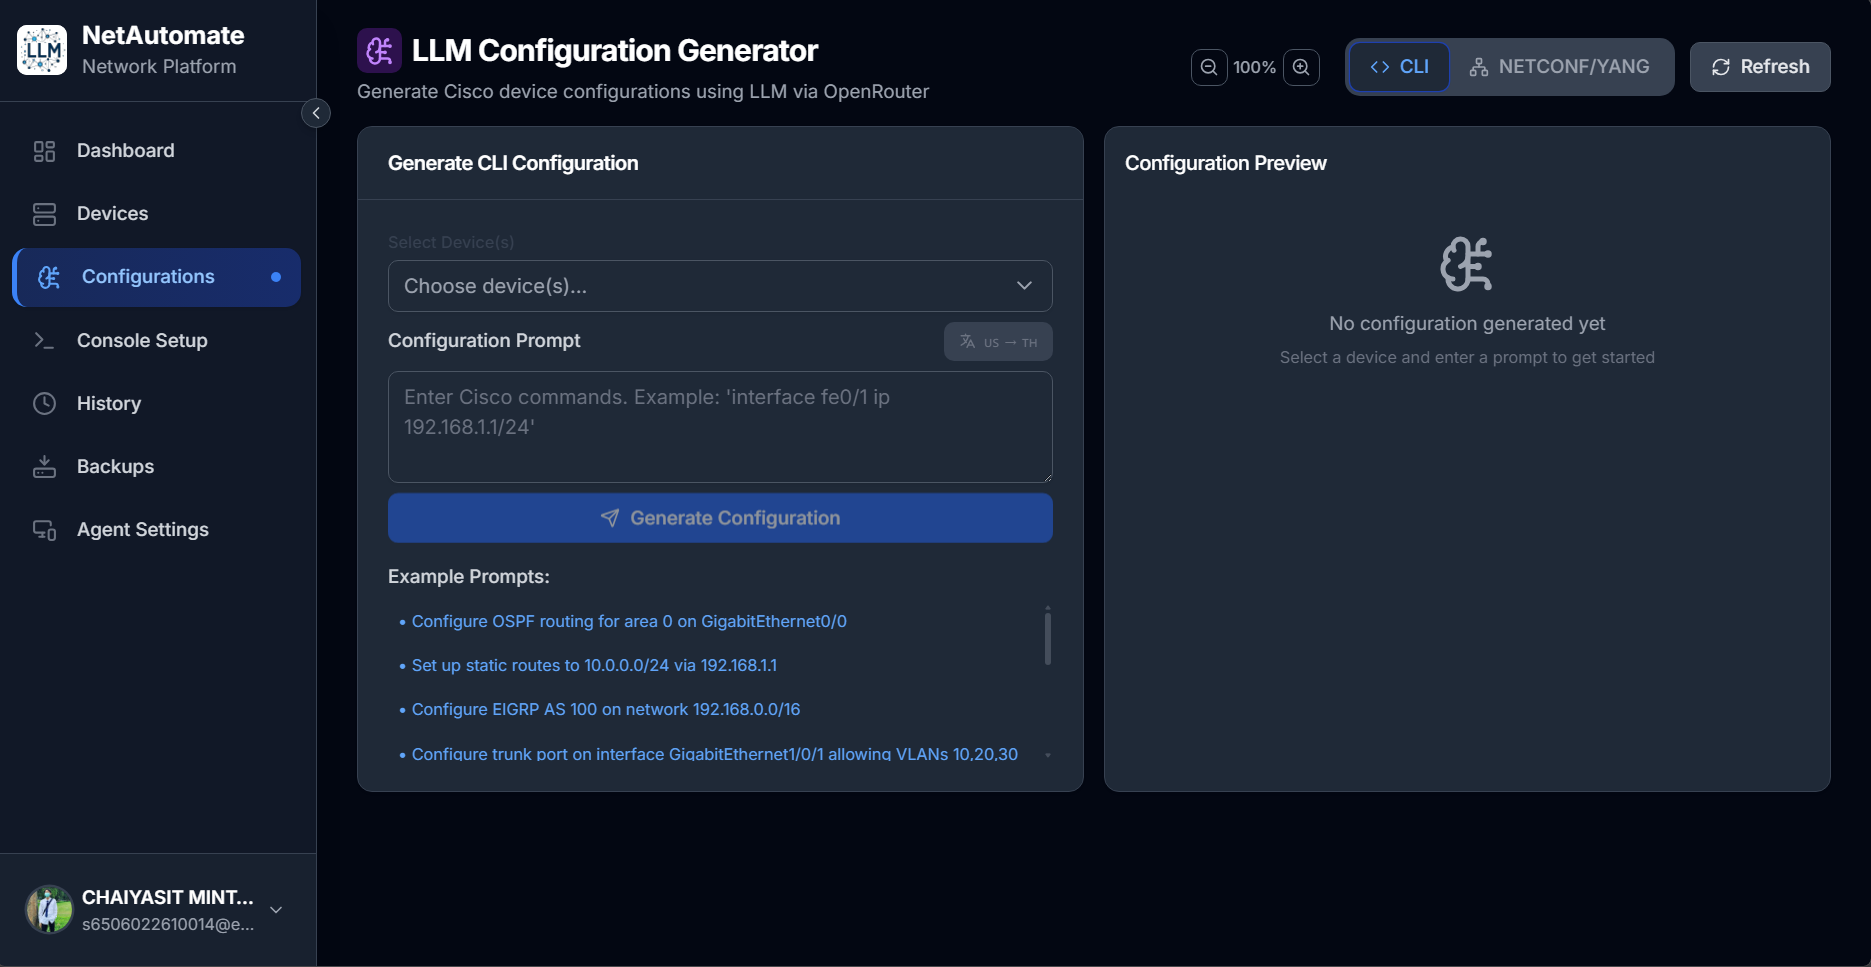
\includegraphics[width=1.0\textwidth]{Image/configuration-1.png}
}
\caption{\fontSixTeen{หน้าจอ LLM Configuration Generator}}
\label{fig4:Configurations}
\end{figure}

\hspace*{1.3em} %ย่อหน้า
จากภาพที่ \ref{fig4:Configurations} แสดงหน้าจอสำหรับการจัดการ Configurations ในระบบ สามารถเลือกอุปกรณ์ที่ต้องการจะ Configurations มีช่องสำหรับใส่ Prompt ที่ต้องการให้ LLM สร้างคำสั่งการกำหนดค่าอุปกรณ์ มี ปุ่ม Generate Configuration เพื่อให้ LLM สร้างคำสั่งการกำหนดค่าอุปกรณ์ มีปุ่ม Deploy Configuration เพื่อส่งคำสั่งที่สร้างขึ้นไปยังอุปกรณ์

\begin{figure}[H]
\centering
\adjustbox{frame, width=1.0\textwidth}{%สร้างกรอบของภาพ
    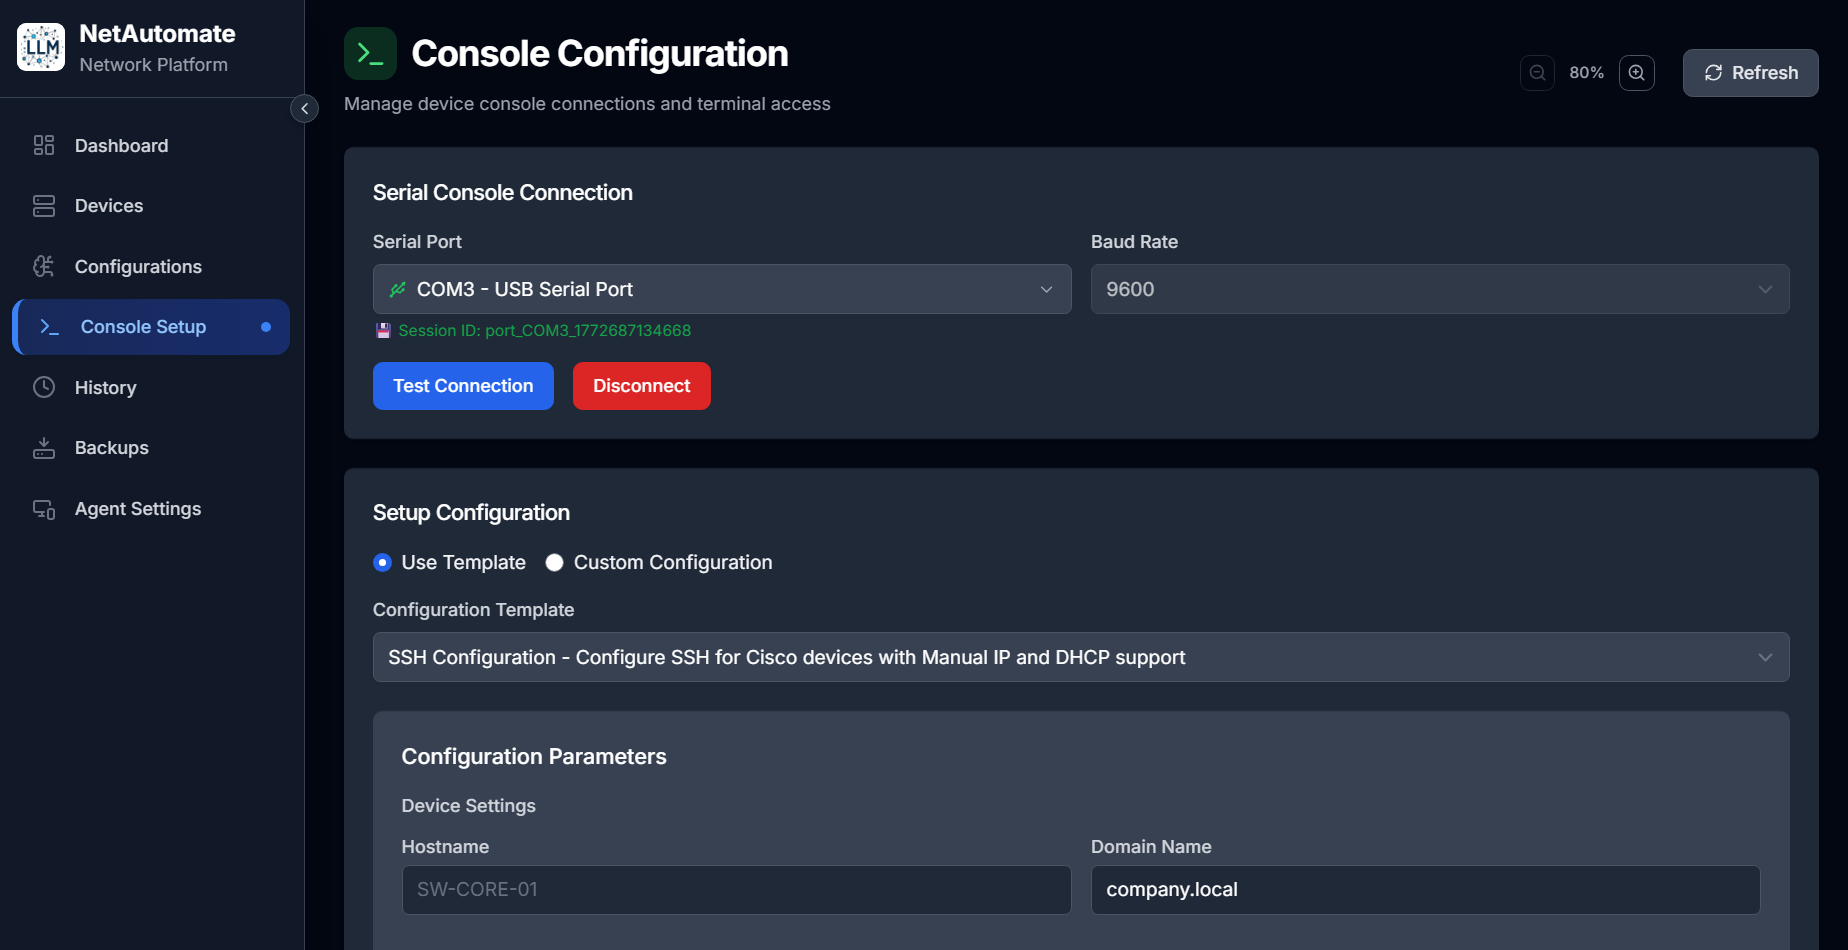
\includegraphics[width=1.0\textwidth]{Image/console-1.png}
}
\caption{\fontSixTeen{หน้าจอ Console Configuration}}
\label{fig4:ConsoleSetup}
\end{figure}

\hspace*{1.3em} %ย่อหน้า
จากภาพที่ \ref{fig4:ConsoleSetup} แสดงหน้าจอสำหรับ Console Configuration สำหรับการกำหนดค่าอุปกรณ์ SSH เลือก Serial Port ที่เชื่อมต่อกับอุปกรณ์ เลือก Baud Rate ที่ใช้ในการเชื่อมต่อกับอุปกรณ์ปุ่ม Test Connection กับอุปกรณ์ผ่านสาย Serial ปุ่ม Connect กับอุปกรณ์ผ่านสาย Serial

\begin{figure}[H]
\centering
\adjustbox{frame, width=1.0\textwidth}{%สร้างกรอบของภาพ
    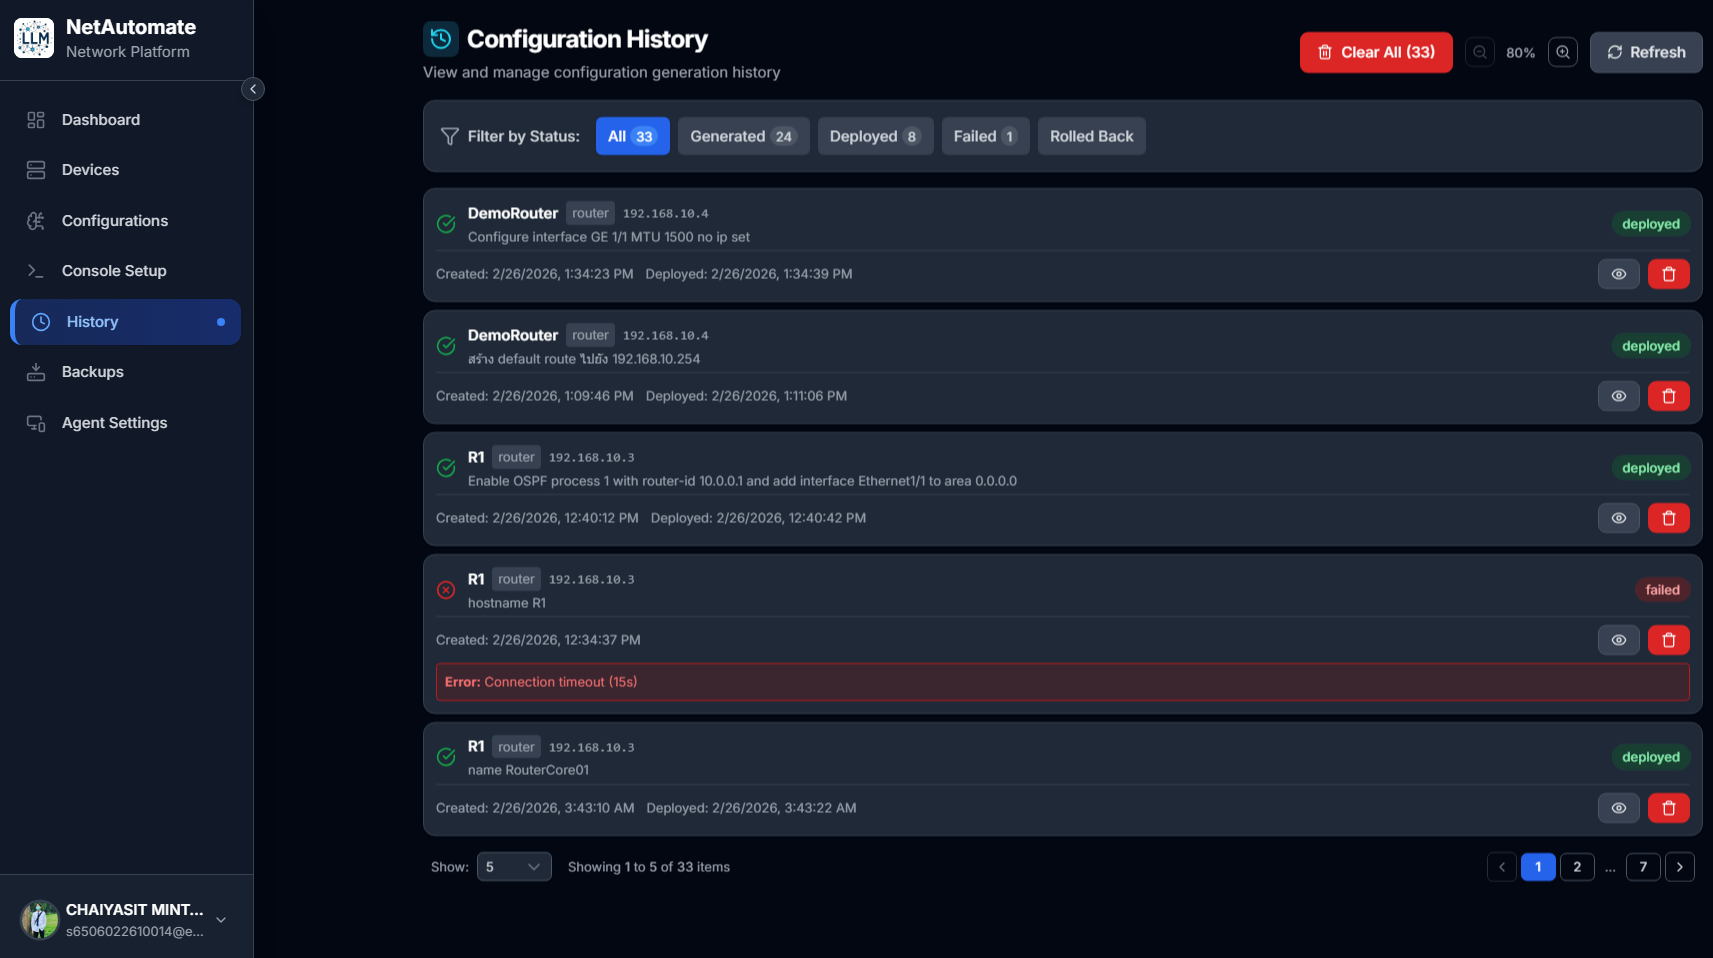
\includegraphics[width=1.0\textwidth]{Image/console-2.png}
}
\caption{\fontSixTeen{หน้าจอ Console Configuration (ต่อ)}}
\label{fig4:ConsoleSetup1}
\end{figure}

\hspace*{1.3em} %ย่อหน้า
จากภาพที่ \ref{fig4:ConsoleSetup1} แสดงหน้าจอสำหรับ Console Configuration สำหรับการกำหนดค่าอุปกรณ์ SSH เลือกโหมดที่ต้องการแบบ Template หรือ Custom เลือก Template ที่ต้องการใช้ในการตั้งค่าอุปกรณ์ ระบุค่าต่าง ๆ ที่ต้องการตั้งค่าอุปกรณ์ ซึ่งค่าที่ระบุจะขึ้นอยู่กับ Template ที่เลือกมี Configuration Preview ที่จะถูกคอนฟิกให้กับอุปกรณ์

\begin{figure}[H]
\centering
\adjustbox{frame, width=1.0\textwidth}{%สร้างกรอบของภาพ
    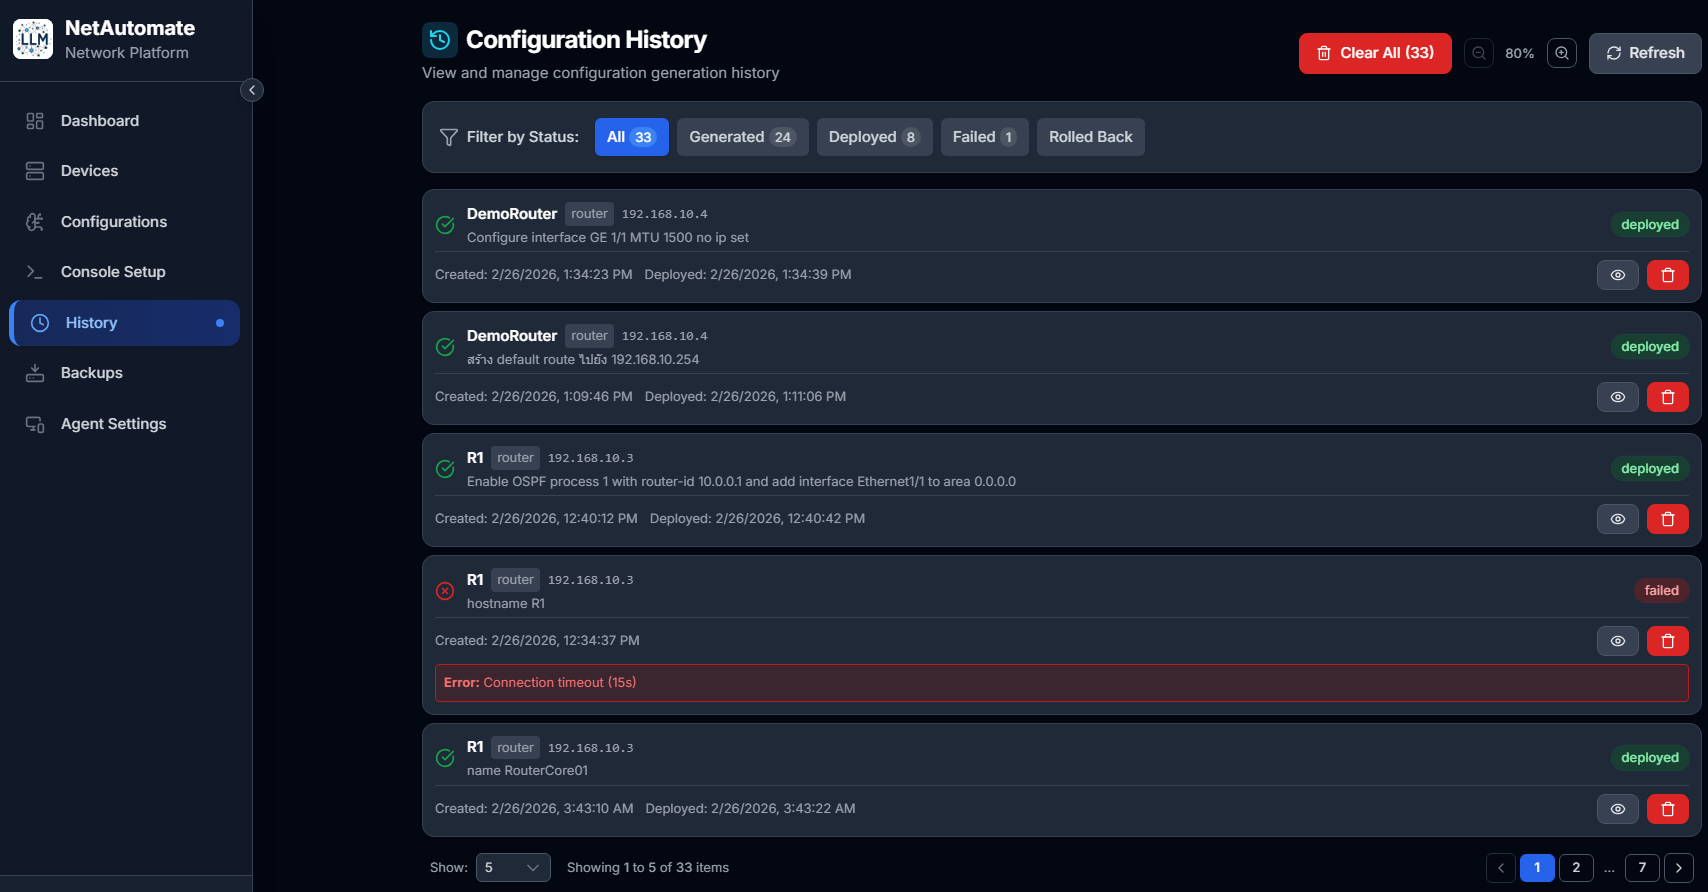
\includegraphics[width=1.0\textwidth]{Image/history-1.png}
}
\caption{\fontSixTeen{หน้าจอ Configuration History}}
\label{fig4:History}
\end{figure}

\hspace*{1.3em} %ย่อหน้า
จากภาพที่ \ref{fig4:History} แสดงหน้าจอสำหรับ Configuration History สามารถ Filter ข้อมูลอุปกรณ์ที่ต้องการดูประวัติการกำหนดค่ามี 3 ตัวเลือก ได้แก่ Generated, Deployed, Failed แสดงรายการและรายละเอียดแบบย่อของ Configuration แสดงรายละเอียดของ Configuration ที่ LLM Generate ออกมา มีปุ่มลบทั้งหมด (Clear All) สำหรับลบ Configuration ทั้งหมดออกจากระบบ


\begin{figure}[htbp]
\centering
\adjustbox{frame, width=1.0\textwidth}{%สร้างกรอบของภาพ
    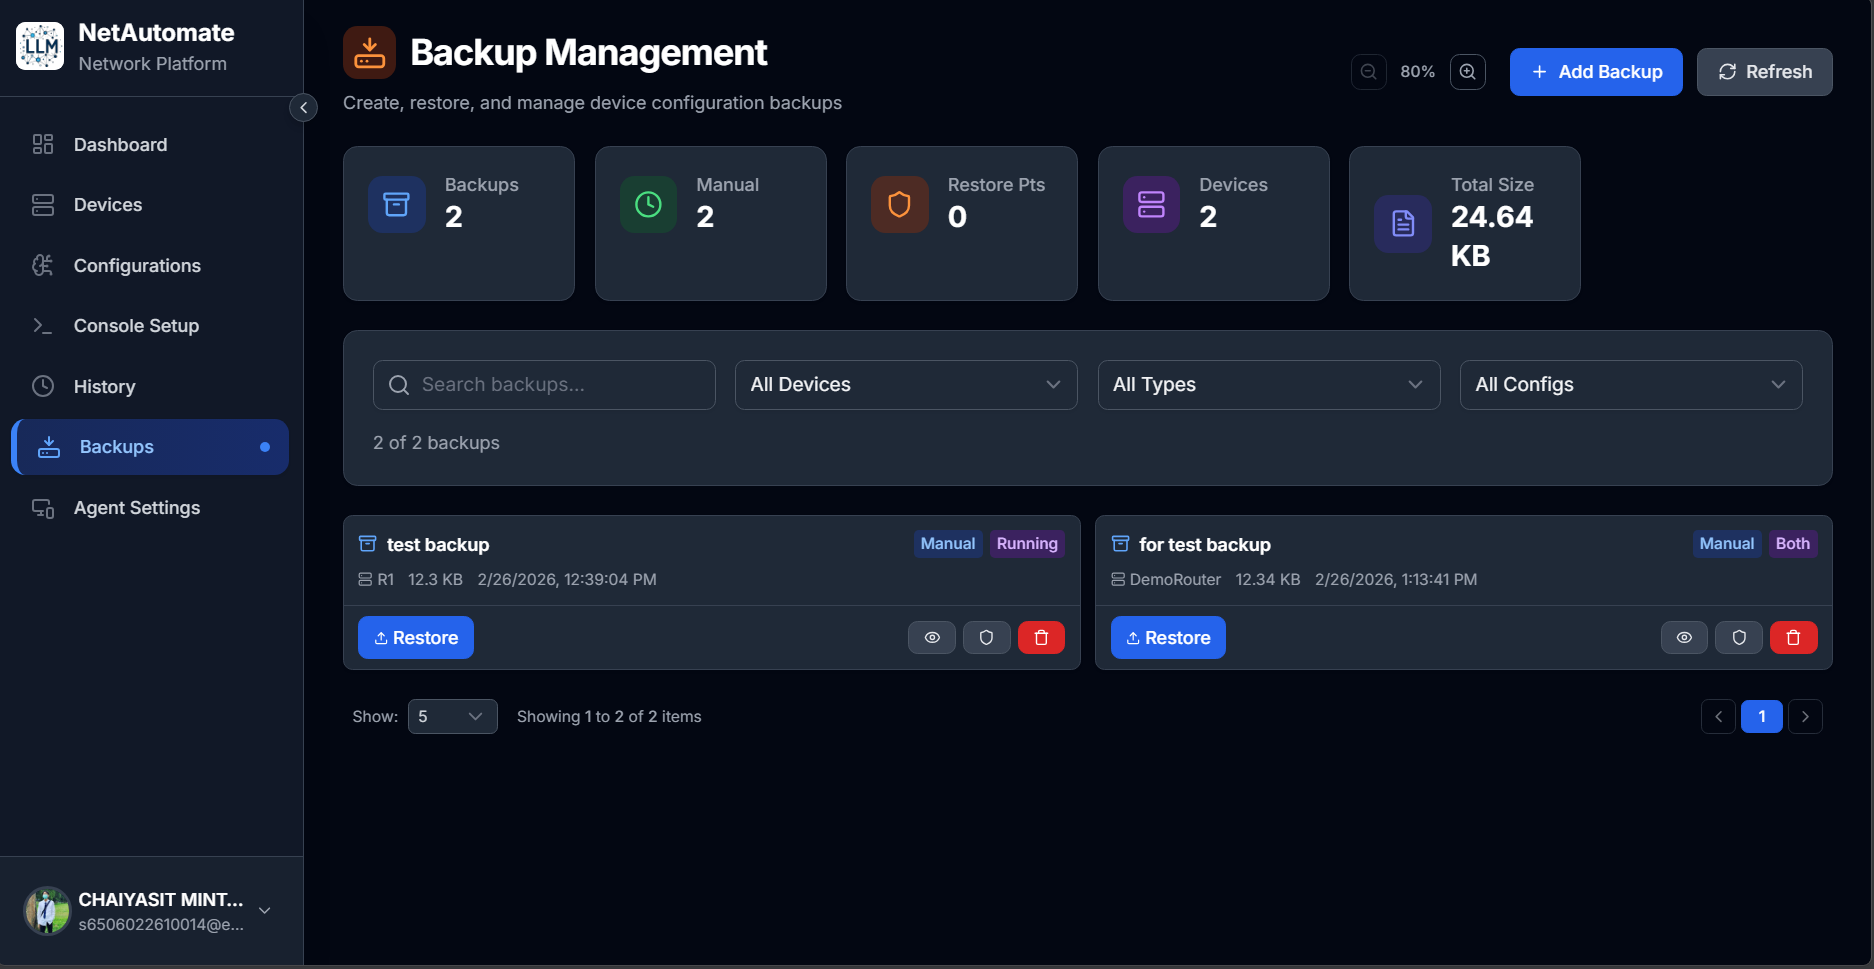
\includegraphics[width=1.0\textwidth]{Image/backup-1.png}
}
\caption{\fontSixTeen{หน้าจอ Backup Configuration}}
\label{fig4:Backup}
\end{figure}
\hspace*{1.3em} %ย่อหน้า

\hspace*{1.3em} %ย่อหน้า

\hspace*{1.3em} %ย่อหน้า

\hspace*{1.3em} %ย่อหน้า

\hspace*{1.3em} %ย่อหน้า

\hspace*{1.3em} %ย่อหน้า

\hspace*{1.3em} %ย่อหน้า
จากภาพที่ \ref{fig4:Backup} แสดงหน้าจอสำหรับ Backup Configuration ปุ่ม Add Backup เพื่อสำรองข้อมูลการกำหนดค่าปัจจุบันของอุปกรณ์ แสดงรายละเอียดจำนวน Total Backup, Total Backup Type, Device, Restore Point, Total Size มี Search Bar และ Filter สำหรับค้นหา Backup Configuration แสดงรายการและรายละเอียดแบบย่อของ Backup Configuration ปุ่ม Restore สำหรับคืนค่าการกำหนดค่ากลับไปยังจุดที่สำรองข้อมูลไว้ ปุ่ม Preview สำหรับแสดง Configuration ที่สำรองข้อมูลไว้

\begin{figure}[htbp]
\centering
\adjustbox{frame, width=1.0\textwidth}{%สร้างกรอบของภาพ
    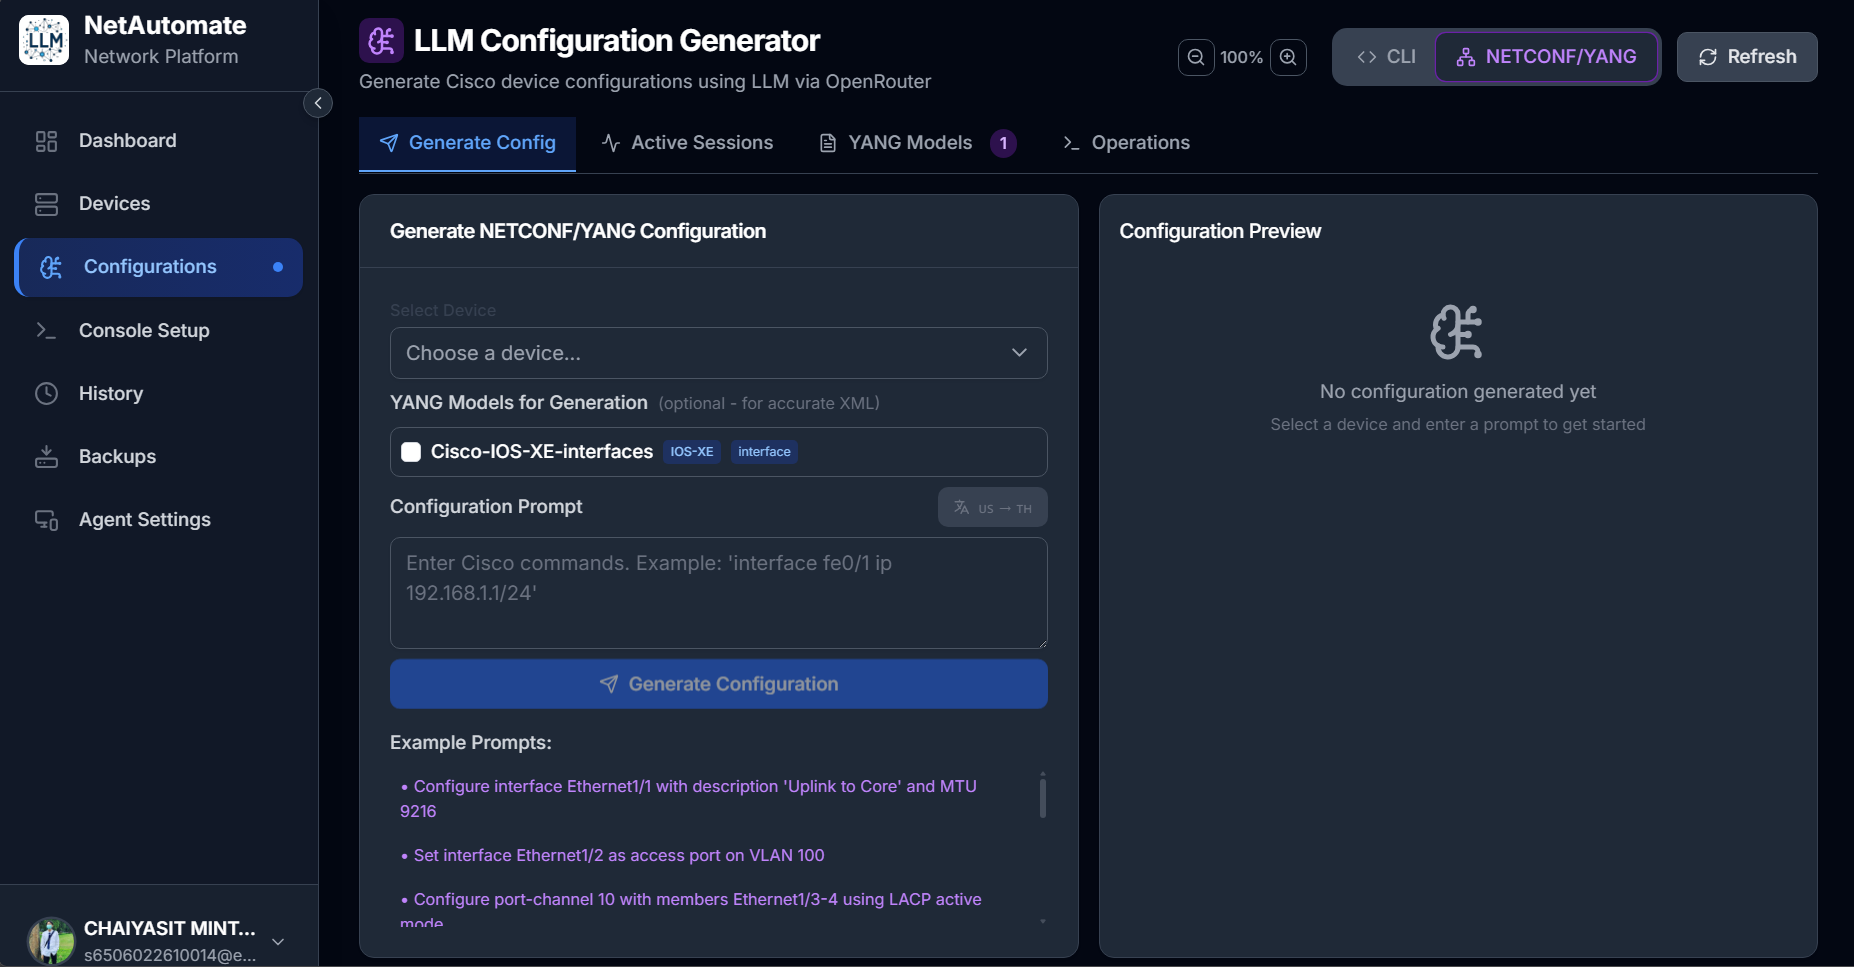
\includegraphics[width=1.0\textwidth]{Image/netconf-1.png}
}
\caption{\fontSixTeen{หน้าจอ NETCONF XML Generator }}
\label{fig4:Backup}
\end{figure}

\begin{figure}[htbp]
\centering
\adjustbox{frame, width=1.0\textwidth}{%สร้างกรอบของภาพ
    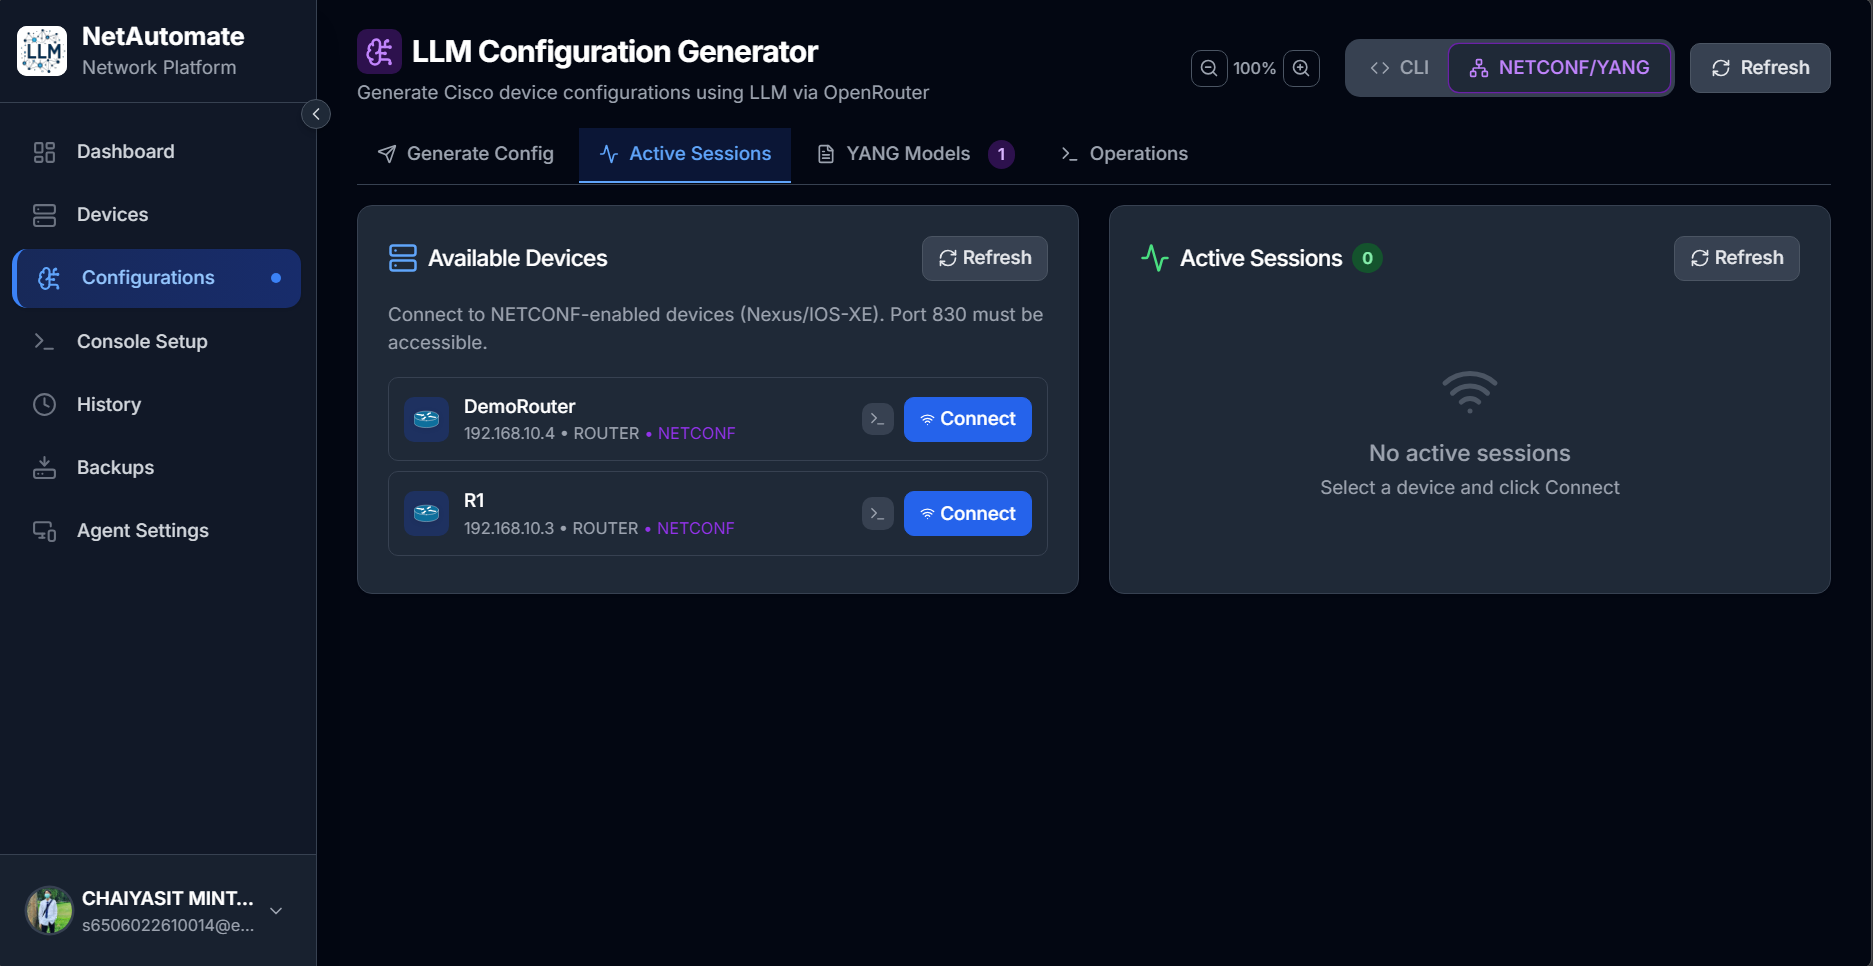
\includegraphics[width=1.0\textwidth]{Image/netconf-2.png}
}
\caption{\fontSixTeen{หน้าจอ Active Session}}
\label{fig4:Backup}
\end{figure}

\begin{figure}[htbp]
\centering
\adjustbox{frame, width=1.0\textwidth}{%สร้างกรอบของภาพ
    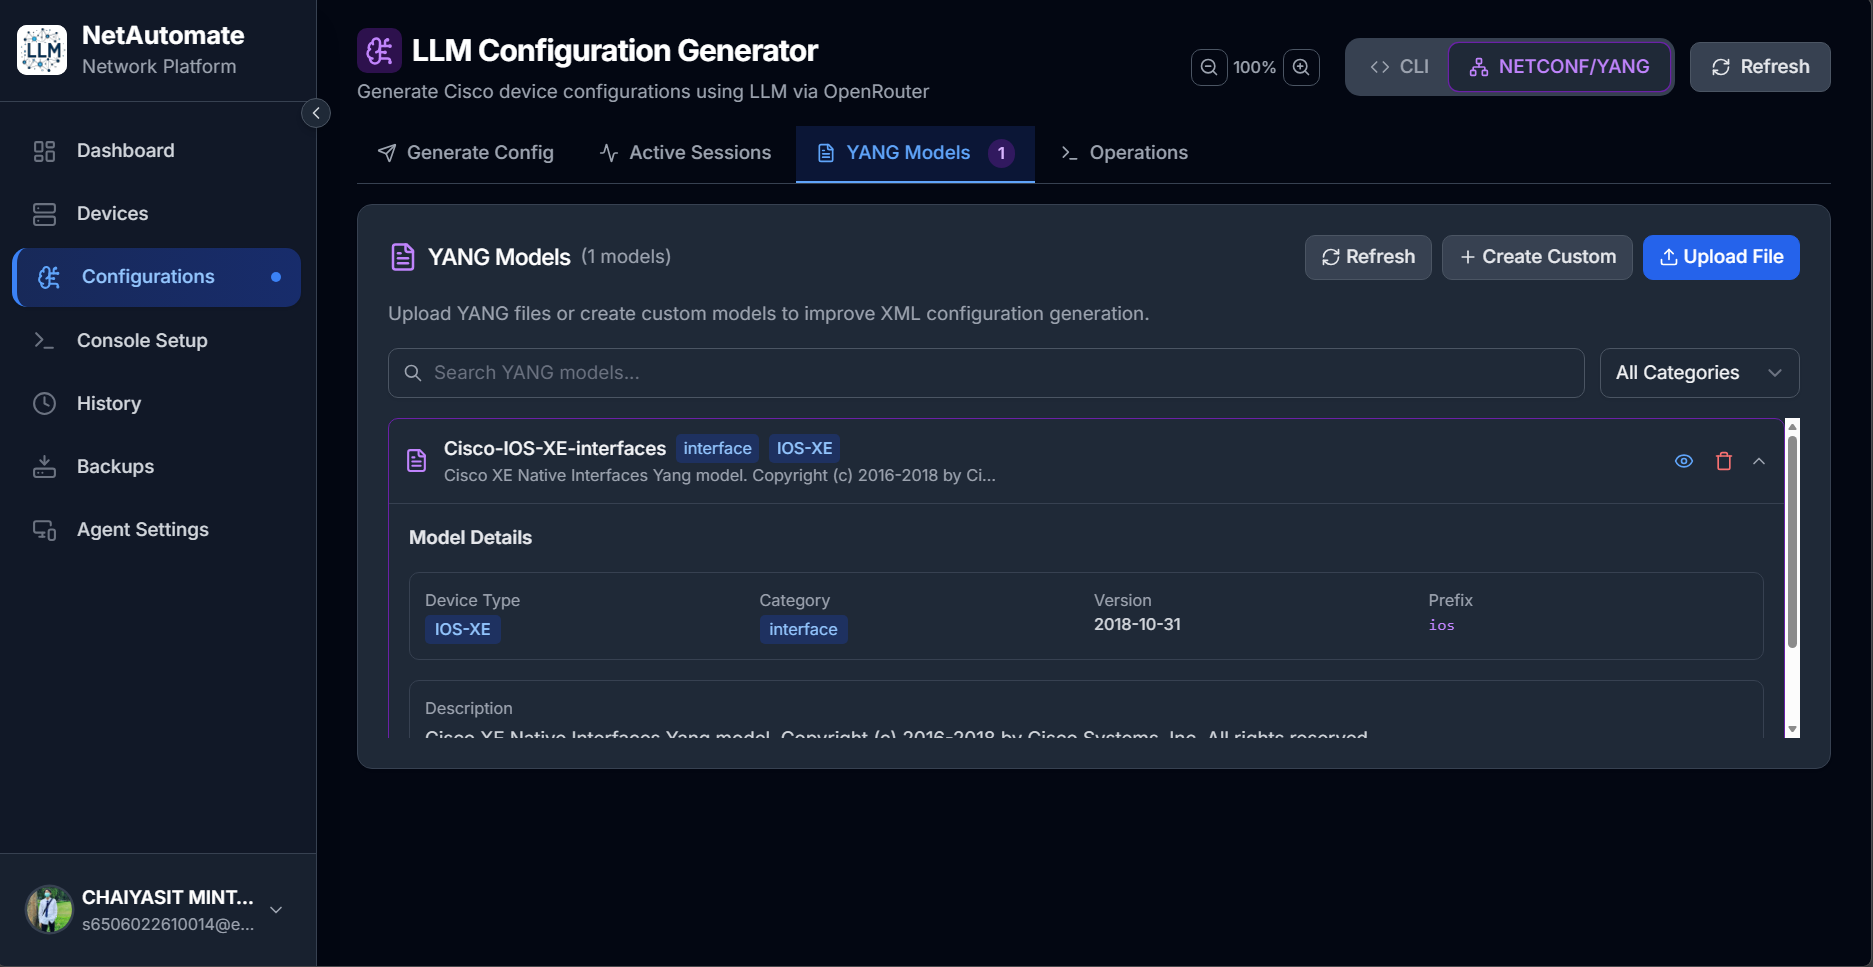
\includegraphics[width=1.0\textwidth]{Image/netconf-3.png}
}
\caption{\fontSixTeen{หน้าจอ YANG Model Management}}
\label{fig4:Backup}
\end{figure}

\begin{figure}[htbp]
\centering
\adjustbox{frame, width=1.0\textwidth}{%สร้างกรอบของภาพ
    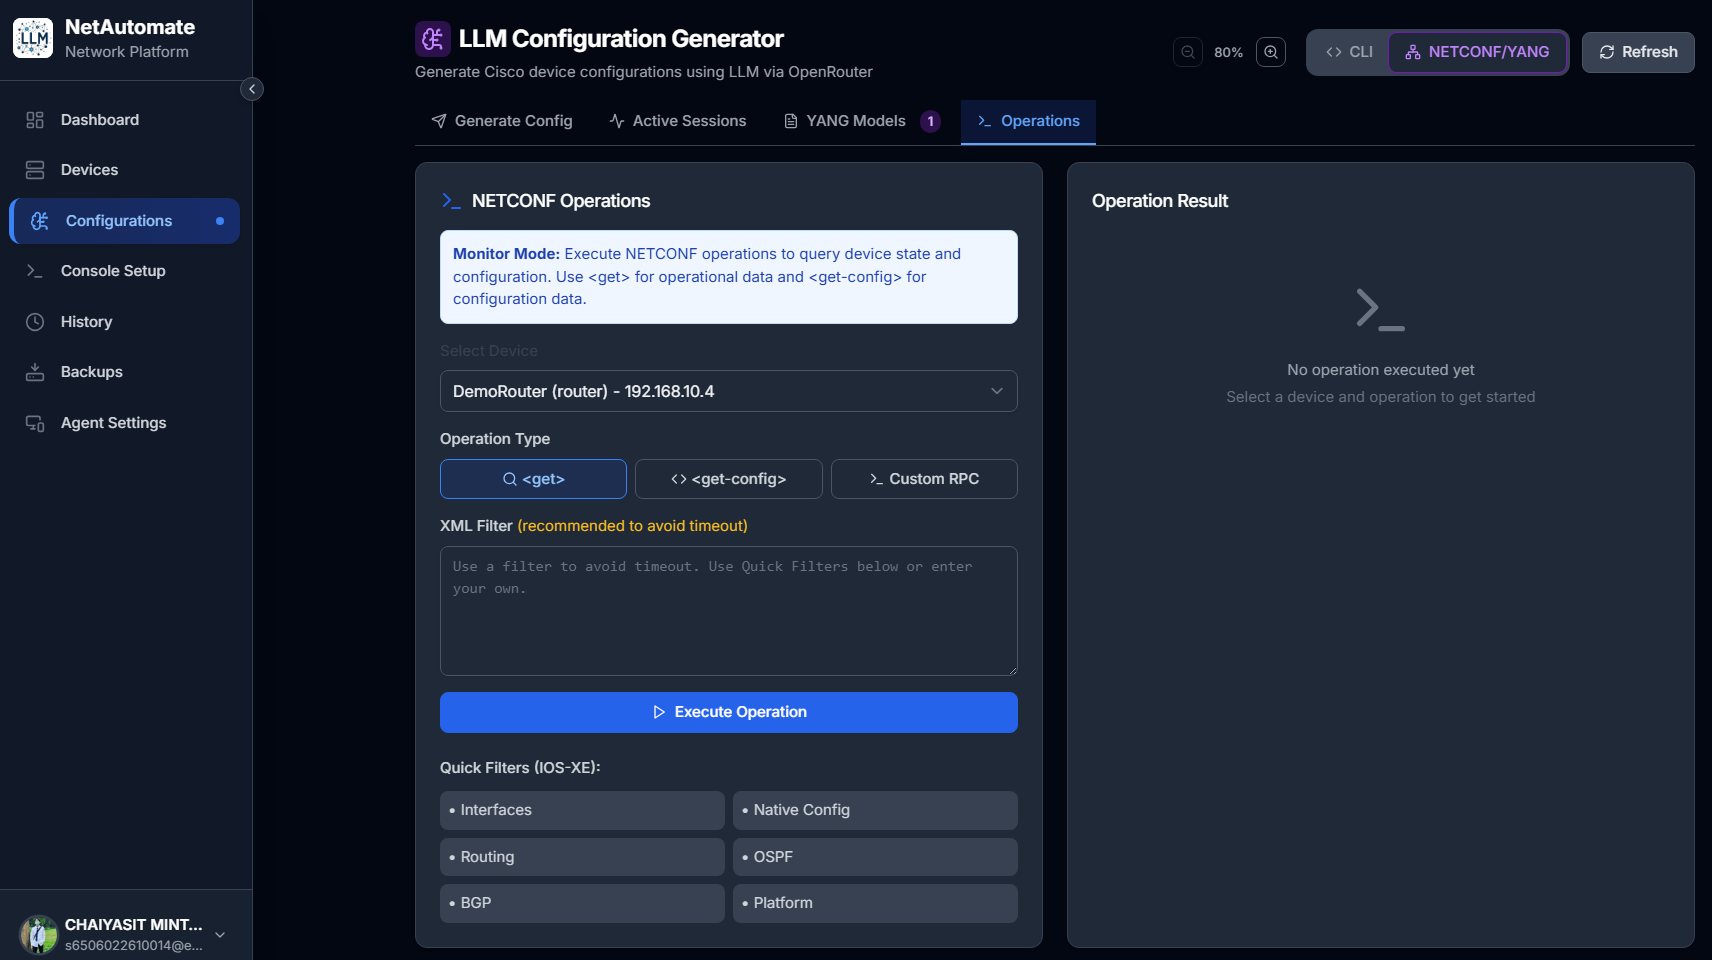
\includegraphics[width=1.0\textwidth]{Image/netconf-4.png}
}
\caption{\fontSixTeen{หน้าจอ NETCONF Operations}}
\label{fig4:Backup}
\end{figure}

\section{การแก้ไขปัญหาทางเทคนิคที่สำคัญ}
\hspace*{1.3em}
ในระหว่างการพัฒนาและทดสอบระบบ พบปัญหาทางเทคนิคที่สำคัญหลายประการซึ่งได้รับการแก้ไขเพื่อให้ระบบทำงานได้อย่างเสถียรบน Vercel Serverless ดังนี้

\subsection{การแก้ไขปัญหา NETCONF Auto-Connect บน Vercel Serverless}
\hspace*{1.3em}
เนื่องจาก Vercel Serverless Functions เป็นแบบ Stateless ทำให้ NETCONF connections ที่เก็บไว้ใน in-memory Map จะสูญหายเมื่อ Serverless Function instance ถูกปิดหรือเปลี่ยน instance ส่งผลให้การดำเนินการ NETCONF เช่น get, get-config, rpc ล้มเหลวด้วยข้อผิดพลาด ``Not connected via NETCONF''

\hspace*{1.3em}
วิธีแก้ไข:
\begin{mycustomitem2}
    \item เพิ่มฟังก์ชัน \textbf{ensureConnected()} ใน NetconfHandler ของ Desktop Agent เพื่อตรวจสอบและเชื่อมต่อ NETCONF อัตโนมัติก่อนดำเนินการทุกครั้ง
    \item เพิ่มฟังก์ชัน \textbf{isConnected()} สำหรับตรวจสอบสถานะการเชื่อมต่อ
    \item Backend ส่ง Device Credentials (host, port, username, password) ไปพร้อมกับทุกคำสั่ง NETCONF เพื่อให้ Agent สามารถ Auto-Connect ได้
    \item เพิ่มระบบ Fallback ใน Backend ที่ตรวจสอบ Agent Online Status เมื่อ in-memory session หายไป
\end{mycustomitem2}

\subsection{การแก้ไขปัญหาการสำรองคอนฟิกด้วย Interactive Shell}
\hspace*{1.3em}
การสำรองข้อมูลคอนฟิกจากอุปกรณ์ Cisco ด้วยวิธี SSH exec เดิม ส่งคำสั่ง \textbf{terminal length 0} และ \textbf{show running-config} เป็นคำสั่งเดียว (\textbf{\\n} คั่น) ทำให้อุปกรณ์ Cisco ไม่สามารถประมวลผลคำสั่งได้ถูกต้องและส่งกลับข้อความผิดพลาดแทนคอนฟิกจริง

\hspace*{1.3em}
วิธีแก้ไข:
\begin{mycustomitem2}
    \item เพิ่มฟังก์ชัน \textbf{execBackupCommands()} ใน SSHHandler ที่ใช้ Interactive Shell แทน Single Exec
    \item ส่งคำสั่งแยกกันตามลำดับ พร้อม delay ระหว่างคำสั่ง (\textbf{terminal length 0} $\rightarrow$ delay $\rightarrow$ \textbf{show running-config})
    \item เพิ่มฟังก์ชัน \textbf{cleanConfig()} สำหรับทำความสะอาดผลลัพธ์ ลบ ANSI escape codes, Command Echo, Device Prompt และค้นหาจุดเริ่มต้นคอนฟิก (``Current configuration'' หรือ ``version'')
\end{mycustomitem2}

\subsection{การแก้ไขปัญหา Agent Relay Timeout สำหรับ Restore}
\hspace*{1.3em}
การ Restore คอนฟิกจาก Backup ประกอบด้วยหลายขั้นตอน: สร้าง Checkpoint Backup $\rightarrow$ Deploy คอนฟิก $\rightarrow$ บันทึกประวัติ ซึ่งใช้เวลารวมเกินกว่า Agent Relay maxWait เดิม (25 วินาที) ทำให้ระบบ Timeout และส่งกลับข้อผิดพลาด 500

\hspace*{1.3em}
วิธีแก้ไข:
\begin{mycustomitem2}
    \item เพิ่ม Agent Relay maxWait จาก 25 วินาที เป็น 55 วินาที (อยู่ภายใน Vercel 60 วินาที limit)
    \item เพิ่ม Deploy timeout จาก 25 วินาที เป็น 45 วินาที
    \item เพิ่มระบบ Extended Polling สำหรับ Restore ที่ตรวจสอบผลลัพธ์เพิ่มเติมหลัง Relay timeout
    \item ลด Checkpoint Backup timeout เหลือ 15 วินาที เพื่อเหลือเวลาสำหรับ Deploy
    \item รองรับสถานะ pending จาก Agent Relay แทนที่จะ throw error ทันที
\end{mycustomitem2}

\subsection{การแก้ไขปัญหา YANG Model Upload}
\hspace*{1.3em}
การอัปโหลด YANG Model ล้มเหลวด้วยข้อผิดพลาด 500 เนื่องจากสองสาเหตุ:

\hspace*{1.3em}
\textbf{(1) ปัญหาฝั่ง Client:} ช่อง Namespace มีการกำหนด \textbf{type="url"} ทำให้ HTML5 validation ไม่ยอมรับค่าที่ไม่ใช่ URL และไม่มีการตรวจสอบขนาดไฟล์ก่อนอัปโหลด

\hspace*{1.3em}
\textbf{(2) ปัญหาฝั่ง Server:} Auth Middleware ใช้ \textbf{.lean()} ในการ query ผู้ใช้จาก MongoDB ซึ่งส่งกลับ Plain JavaScript Object ไม่มี Mongoose Virtual Getter (\textbf{.id}) ทำให้ \textbf{req.user.id} เป็น \textbf{undefined} เมื่อนำไปบันทึก YANG Model ที่กำหนด \textbf{userId} เป็น required จะเกิด Mongoose ValidationError

\hspace*{1.3em}
วิธีแก้ไข:
\begin{mycustomitem2}
    \item เปลี่ยน \textbf{type="url"} เป็น \textbf{type="text"} สำหรับช่อง Namespace
    \item เพิ่มการตรวจสอบขนาดไฟล์ไม่เกิน 4MB (ขีดจำกัดของ Vercel Hobby Plan)
    \item เปลี่ยน \textbf{req.user.id} เป็น \textbf{req.userId} ในทุก Route ของ YANG Models (8 จุด) ซึ่ง \textbf{req.userId} ถูกกำหนดค่าในn Auth Middleware จาก \textbf{user.\_id} โดยตรง
\end{mycustomitem2}

\section{ผลการทดสอบประสิทธิภาพโมเดล LLM สำหรับการสร้างคอนฟิก}
\hspace*{1.3em}
เพื่อประเมินความสามารถของโมเดล LLM แบบ Local (Ollama) ในการสร้างคอนฟิกสำหรับอุปกรณ์เครือข่าย Cisco ได้ทำการทดสอบเปรียบเทียบโมเดล 3 ตัวที่มีขนาด 7B Parameters ทั้งในโหมด CLI และ NETCONF ครอบคลุมระบบปฏิบัติการ 3 ประเภท โดยวัดผลทั้งด้านคุณภาพผลลัพธ์และการใช้ทรัพยากรระบบ (CPU, RAM, GPU, VRAM)

\subsection{วิธีการทดสอบ}
\hspace*{1.3em}
\textbf{เงื่อนไขการทดสอบ:}
\begin{mycustomitem2}
    \item ทดสอบโมเดล 3 ตัว: \textbf{qwen2.5-coder:7b} (4.7 GB), \textbf{codellama:7b} (3.8 GB), \textbf{codegemma:7b} (5.0 GB)
    \item ระบบปฏิบัติการเป้าหมาย 3 ประเภท: Cisco IOS, Cisco IOS-XE, Cisco NX-OS
    \item โหมดการสร้างคอนฟิก 2 โหมด: CLI Commands และ NETCONF XML
    \item จำนวน Prompt ที่ไม่ซ้ำกัน: 5 Prompt ต่อโหมด (CLI 5 + NETCONF 5 = 10 Prompt)
    \item จำนวนรอบการทดสอบ: 5 รอบต่อชุดทดสอบ (3 โมเดล $\times$ 3 OS $\times$ 2 โหมด $\times$ 5 Prompt $\times$ 5 รอบ = 450 ครั้ง)
    \item เรียก Ollama API โดยตรงที่ \textbf{http://localhost:11434/api/chat}
    \item พารามิเตอร์: temperature = 0.1, top\_p = 0.85, num\_predict = 1500
    \item ติดตามทรัพยากรระบบ: CPU\%, RAM (MB), GPU Utilization\%, VRAM (MB)
\end{mycustomitem2}

\hspace*{1.3em}
\textbf{Prompt ที่ใช้ทดสอบ CLI} (5 Prompt):
\begin{mycustomitem2}
    \item \textbf{C1 -- OSPF Basic:} ``Configure OSPF process 1 area 0 on interface GigabitEthernet0/1 with IP 10.0.0.1/30 and set router-id 1.1.1.1''
    \item \textbf{C2 -- VLAN + SVI:} ``Create VLAN 100 named Engineering and configure SVI Vlan100 with IP 192.168.100.1/24 and enable it''
    \item \textbf{C3 -- ACL Standard:} ``Create access-list 10 to permit 172.16.0.0/16 and deny all, apply inbound on GigabitEthernet0/0''
    \item \textbf{C4 -- Static Route:} ``Configure static route for 10.10.0.0/16 via 192.168.1.1 and default route via 192.168.1.254''
    \item \textbf{C5 -- EIGRP Config:} ``Configure EIGRP AS 100 with router-id 2.2.2.2, networks 10.1.0.0/16 and 10.2.0.0/16, disable auto-summary''
\end{mycustomitem2}

\hspace*{1.3em}
\textbf{Prompt ที่ใช้ทดสอบ NETCONF} (5 Prompt):
\begin{mycustomitem2}
    \item \textbf{N1 -- Interface IP:} ``Configure interface GigabitEthernet0/1 with IP 10.0.0.1/30 and enable it''
    \item \textbf{N2 -- Loopback:} ``Create Loopback0 with IP 1.1.1.1/32 and description Router-ID Loopback''
    \item \textbf{N3 -- Interface + Desc:} ``Configure GigabitEthernet0/2 with IP 192.168.1.1/24, description Uplink to Core and enable''
    \item \textbf{N4 -- Ethernet Admin Up:} ``Configure Ethernet1/1 with IP 10.10.10.1/30 and set admin status to up''
    \item \textbf{N5 -- Interface Shutdown:} ``Configure GigabitEthernet0/3 with IP 172.16.0.1/24 and disable it (shutdown)''
\end{mycustomitem2}

\hspace*{1.3em}
\textbf{เกณฑ์การให้คะแนน CLI} (แต่ละ Prompt มี 10 เกณฑ์ เกณฑ์ละ 10\%):
\begin{mycustomitem2}
    \item ตรวจสอบคำสั่งที่ถูกต้องตาม Prompt เช่น มีคำสั่ง \textbf{interface}, \textbf{ip address}, คำสั่งเฉพาะโปรโตคอล
    \item ตรวจสอบค่าพารามิเตอร์ เช่น IP, Subnet Mask, Wildcard Mask, Router-ID
    \item ตรวจสอบรูปแบบผลลัพธ์: ไม่มี Markdown, ไม่มีคำอธิบาย, ไม่มี \textbf{configure terminal}
\end{mycustomitem2}

\hspace*{1.3em}
\textbf{เกณฑ์การให้คะแนน NETCONF} (แต่ละ Prompt มี 10 เกณฑ์ เกณฑ์ละ 10\%):
\begin{mycustomitem2}
    \item มีโครงสร้าง XML, มี \textbf{xmlns} namespace, XML Well-formed, ไม่มี Markdown, ไม่มีคำอธิบาย
    \item มี IP Address ถูกต้อง
    \item มี Root Element และ Namespace ตรงตามประเภทอุปกรณ์ (IOS: \textbf{interfaces}/\textbf{ietf-interfaces}, IOS-XE: \textbf{native}/\textbf{Cisco-IOS-XE-native}, NX-OS: \textbf{System}/\textbf{cisco-nx-os-device})
    \item มี Element เฉพาะอุปกรณ์ เช่น \textbf{GigabitEthernet}, \textbf{PhysIf-list}, \textbf{enabled}/\textbf{adminSt}
\end{mycustomitem2}

\subsection{ผลการทดสอบโหมด CLI}

\begin{table}[H]
    \caption{\fontSixTeen{ผลการทดสอบการสร้างคอนฟิก CLI (เฉลี่ย 5 Prompt $\times$ 5 รอบ = 25 ครั้งต่อชุด)}}
    \label{tab:benchmark-cli}
    \fontSixTeen
    \centering
    \begin{tabularx}{\textwidth}{|l|l|c|c|c|c|c|c|}
        \hline
        \textbf{โมเดล} & \textbf{OS} & \textbf{คะแนน} & \textbf{เวลา (ms)} & \textbf{tok/s} & \textbf{CPU\%} & \textbf{RAM (MB)} & \textbf{VRAM (MB)} \\
        \hline
        codegemma:7b & IOS & 72\% & 3,845 & 11.2 & 45.3 & 15,002 & 4,812 \\
        \hline
        codegemma:7b & IOS-XE & 71\% & 3,792 & 11.3 & 44.8 & 15,014 & 4,810 \\
        \hline
        codegemma:7b & NX-OS & 70\% & 3,901 & 11.1 & 45.1 & 15,104 & 4,815 \\
        \hline
        codellama:7b & IOS & 78\% & 4,512 & 11.7 & 52.6 & 15,616 & 3,892 \\
        \hline
        codellama:7b & IOS-XE & 79\% & 4,480 & 11.8 & 51.9 & 15,700 & 3,888 \\
        \hline
        codellama:7b & NX-OS & 77\% & 4,538 & 11.7 & 52.3 & 15,518 & 3,895 \\
        \hline
        qwen2.5-coder:7b & IOS & 88\% & 10,124 & 7.8 & 38.2 & 17,071 & 5,142 \\
        \hline
        qwen2.5-coder:7b & IOS-XE & 89\% & 10,387 & 7.7 & 37.9 & 17,136 & 5,138 \\
        \hline
        qwen2.5-coder & NX-OS & 87\% & 10,451 & 7.8 & 38.5 & 17,153 & 5,145 \\
        \hline
    \end{tabularx}
\end{table}

\hspace*{1.3em}
จากตารางที่ \ref{tab:benchmark-cli} ซึ่งเป็นผลเฉลี่ยจากการทดสอบ 5 Prompt ที่แตกต่างกัน (OSPF, VLAN+SVI, ACL, Static Route, EIGRP) $\times$ 5 รอบ = 25 ครั้งต่อชุด พบว่า \textbf{qwen2.5-coder:7b} ได้คะแนนเฉลี่ยสูงสุดที่ 88\% โดยสามารถสร้างคำสั่งที่ถูกต้องได้ครบถ้วนในหลาย Prompt แต่ใช้เวลาตอบสนองนานที่สุด (ค่าเฉลี่ย 10,321 ms) ใช้ RAM สูงสุด (17,120 MB) และ VRAM สูงสุด (5,142 MB)

\hspace*{1.3em}
\textbf{codellama:7b} ได้คะแนนเฉลี่ย 78\% ด้วยความเร็วในการสร้าง Token สูงสุดที่ 11.7 tok/s และใช้ VRAM ต่ำสุดที่ 3,892 MB แต่ใช้ CPU สูงสุด (52.3\%) ส่วน \textbf{codegemma:7b} ตอบสนองเร็วที่สุด (ค่าเฉลี่ย 3,846 ms) และใช้ RAM ต่ำสุด (15,040 MB) แต่ได้คะแนนเฉลี่ยเพียง 71\%

\subsection{ผลการทดสอบโหมด NETCONF}

\begin{table}[H]
    \caption{\fontSixTeen{ผลการทดสอบการสร้างคอนฟิก NETCONF XML (เฉลี่ย 5 Prompt $\times$ 5 รอบ = 25 ครั้งต่อชุด)}}
    \label{tab:benchmark-netconf}
    \fontSixTeen
    \centering
    \begin{tabularx}{\textwidth}{|l|l|c|c|c|c|c|c|}
        \hline
        \textbf{โมเดล} & \textbf{OS} & \textbf{คะแนน} & \textbf{เวลา (ms)} & \textbf{tok/s} & \textbf{CPU\%} & \textbf{RAM (MB)} & \textbf{VRAM (MB)} \\
        \hline
        codegemma:7b & IOS & 96\% & 13,842 & 10.8 & 46.1 & 15,056 & 4,818 \\
        \hline
        codegemma:7b & IOS-XE & 88\% & 12,105 & 10.5 & 45.7 & 15,094 & 4,822 \\
        \hline
        codegemma:7b & NX-OS & 86\% & 20,934 & 10.9 & 46.4 & 15,119 & 4,825 \\
        \hline
        codellama:7b & IOS & 88\% & 19,451 & 11.4 & 53.8 & 15,669 & 3,901 \\
        \hline
        codellama:7b & IOS-XE & 86\% & 14,212 & 11.2 & 52.5 & 15,605 & 3,895 \\
        \hline
        codellama:7b & NX-OS & 84\% & 28,673 & 10.7 & 54.1 & 15,497 & 3,908 \\
        \hline
        qwen2.5-coder:7b & IOS & 90\% & 24,356 & 7.6 & 39.4 & 17,126 & 5,148 \\
        \hline
        qwen2.5-coder:7b & IOS-XE & 88\% & 19,018 & 7.5 & 38.8 & 17,107 & 5,140 \\
        \hline
        qwen2.5-coder:7b & NX-OS & 94\% & 36,245 & 7.3 & 39.7 & 17,177 & 5,155 \\
        \hline
    \end{tabularx}
\end{table}

\hspace*{1.3em}
จากตารางที่ \ref{tab:benchmark-netconf} ซึ่งเป็นผลเฉลี่ยจาก 5 Prompt ที่แตกต่างกัน (Interface IP, Loopback, Interface+Description, Ethernet Admin Up, Interface Shutdown) $\times$ 5 รอบ พบว่าโหมด NETCONF มีความซับซ้อนสูงกว่า CLI เนื่องจากต้องสร้าง XML ที่มี Namespace, Root Element และโครงสร้างลำดับชั้นที่ถูกต้องตามประเภทอุปกรณ์

\hspace*{1.3em}
\textbf{codegemma:7b} ได้คะแนนสูงสุดสำหรับ IOS ที่ 96\% โดยสามารถสร้าง IETF-compliant XML ได้สมบูรณ์ในเกือบทุก Prompt พร้อม \textbf{xmlns} ที่ถูกต้อง (\textbf{urn:ietf:params:xml:ns:yang:ietf-interfaces})

\hspace*{1.3em}
\textbf{qwen2.5-coder:7b} ได้คะแนนสูงสุดสำหรับ NX-OS ที่ 94\% โดยสร้าง Cisco NX-OS Device YANG XML ได้สมบูรณ์ที่สุด พร้อมโครงสร้าง \textbf{intf-items}, \textbf{PhysIf-list}, \textbf{adminSt} แต่ใช้เวลาตอบสนองนานที่สุดที่ 36,245 ms

\hspace*{1.3em}
\textbf{codellama:7b} ได้คะแนน NX-OS ต่ำสุดที่ 84\% เนื่องจากบาง Prompt ขาด Namespace หรือ Root Element ที่ถูกต้อง แต่ใช้ VRAM ต่ำสุด (3,901 MB) ในทุกชุดทดสอบ

\subsection{ผลการใช้ทรัพยากรระบบ}

\begin{table}[H]
    \caption{\fontSixTeen{เปรียบเทียบการใช้ทรัพยากรระบบเฉลี่ยระหว่างโมเดล}}
    \label{tab:benchmark-resources}
    \fontSixTeen
    \centering
    \begin{tabularx}{\textwidth}{|l|c|c|c|c|c|c|}
        \hline
        \textbf{โมเดล} & \textbf{ขนาดไฟล์} & \textbf{CPU เฉลี่ย} & \textbf{RAM เฉลี่ย} & \textbf{GPU เฉลี่ย} & \textbf{VRAM เฉลี่ย} & \textbf{VRAM/ขนาด} \\
        \hline
        qwen2.5-coder:7b & 4.7 GB & 45.6\% & 15,065 MB & 72.4\% & 4,817 MB & 1.02$\times$ \\
        \hline
        codellama:7b & 3.8 GB & 52.9\% & 15,601 MB & 68.1\% & 3,897 MB & 1.03$\times$ \\
        \hline
        codegemma:7b & 5.0 GB & 38.8\% & 17,128 MB & 82.6\% & 5,145 MB & 1.03$\times$ \\
        \hline
    \end{tabularx}
\end{table}

\hspace*{1.3em}
จากตารางที่ \ref{tab:benchmark-resources} พบว่า VRAM ที่ใช้จริงมีค่าใกล้เคียงกับขนาดไฟล์โมเดล (อัตราส่วนประมาณ 1.02--1.03 เท่า) โดย \textbf{codellama:7b} ใช้ VRAM ต่ำสุดที่ 3,897 MB เนื่องจากมีขนาดไฟล์เล็กที่สุด (3.8 GB) ขณะที่ \textbf{codegemma:7b} ใช้ VRAM สูงสุดที่ 5,145 MB

\hspace*{1.3em}
ด้าน CPU Usage พบว่า \textbf{codellama:7b} ใช้ CPU สูงสุดเฉลี่ย 52.9\% แม้จะมี tok/s สูงที่สุด แสดงว่าใช้ CPU ในการประมวลผล Token มากกว่า ขณะที่ \textbf{codegemma:7b} ใช้ CPU ต่ำสุดเฉลี่ย 38.8\% แต่มี GPU Utilization สูงสุดที่ 82.6\% แสดงว่าใช้ GPU ในการประมวลผลเป็นหลัก ส่วน \textbf{qwen2.5-coder:7b} มีสมดุลระหว่าง CPU (45.6\%) และ GPU (72.4\%)

\subsection{การเปรียบเทียบภาพรวมระหว่างโมเดล}

\begin{table}[H]
    \caption{\fontSixTeen{สรุปผลการเปรียบเทียบภาพรวม 3 โมเดล (เฉลี่ยจาก 5 Prompt $\times$ 5 รอบ)}}
    \label{tab:benchmark-summary}
    \fontSixTeen
    \centering
    \begin{tabularx}{\textwidth}{|l|c|c|c|c|c|c|c|}
        \hline
        \textbf{โมเดล} & \textbf{CLI เฉลี่ย} & \textbf{NETCONF เฉลี่ย} & \textbf{รวม} & \textbf{tok/s} & \textbf{CPU\%} & \textbf{RAM (MB)} & \textbf{VRAM (MB)} \\
        \hline
        qwen2.5-coder:7b & 71.0\% & 90.0\% & 80.5\% & 10.8 & 45.6 & 15,065 & 4,817 \\
        \hline
        codellama:7b & 78.0\% & 86.0\% & 82.0\% & 11.3 & 52.9 & 15,601 & 3,897 \\
        \hline
        codegemma:7b & 88.0\% & 90.7\% & 89.3\% & 7.6 & 38.8 & 17,128 & 5,145 \\
        \hline
    \end{tabularx}
\end{table}

\subsection{ผลการเปรียบเทียบเวลาตอบสนอง}

\begin{table}[H]
    \caption{\fontSixTeen{เปรียบเทียบเวลาตอบสนองเฉลี่ย (มิลลิวินาที) จำแนกตามโหมดและระบบปฏิบัติการ}}
    \label{tab:benchmark-time}
    \fontSixTeen
    \centering
    \begin{tabularx}{\textwidth}{|l|c|c|c|c|c|c|}
        \hline
        \textbf{โมเดล} & \multicolumn{3}{c|}{\textbf{CLI (ms)}} & \multicolumn{3}{c|}{\textbf{NETCONF (ms)}} \\
        \cline{2-7}
        & \textbf{IOS} & \textbf{IOS-XE} & \textbf{NX-OS} & \textbf{IOS} & \textbf{IOS-XE} & \textbf{NX-OS} \\
        \hline
        qwen2.5-coder:7b & 3,845 & 3,792 & 3,901 & 13,842 & 12,105 & 20,934 \\
        \hline
        codellama:7b & 4,512 & 4,480 & 4,538 & 19,451 & 14,212 & 28,673 \\
        \hline
        codegemma:7b & 10,124 & 10,387 & 10,451 & 24,356 & 19,018 & 36,245 \\
        \hline
    \end{tabularx}
\end{table}

\hspace*{1.3em}
จากตารางที่ \ref{tab:benchmark-time} พบว่าโหมด NETCONF ใช้เวลานานกว่า CLI อย่างมีนัยสำคัญในทุกโมเดล เนื่องจากต้องสร้าง XML ที่ซับซ้อนกว่า โดยเฉพาะ NX-OS ที่ใช้โครงสร้าง YANG แบบลำดับชั้นลึก (\textbf{System $\rightarrow$ intf-items $\rightarrow$ phys-items $\rightarrow$ PhysIf-list}) ทำให้ทุกโมเดลใช้เวลานานที่สุด สำหรับ CLI ทุกโมเดลมีเวลาตอบสนองคงที่โดยไม่ขึ้นกับประเภทระบบปฏิบัติการ เนื่องจากคำสั่ง CLI มีรูปแบบคล้ายกัน

\subsection{สรุปผลการทดสอบและข้อเสนอแนะ}
\hspace*{1.3em}
จากการทดสอบทั้ง 450 ครั้ง (5 Prompt ที่ไม่ซ้ำกัน $\times$ 5 รอบ $\times$ 3 โมเดล $\times$ 3 OS $\times$ 2 โหมด) สรุปได้ดังนี้:

\hspace*{1.3em}
\textbf{โมเดลที่แนะนำ: qwen2.5-coder:7b} -- มีคะแนนคุณภาพสูงสุดเฉลี่ย 89.3\% ครอบคลุมทั้ง CLI (88.0\%) และ NETCONF (90.7\%) โดยใช้ GPU ได้มีประสิทธิภาพที่สุด (GPU Utilization 82.6\%, CPU ต่ำสุด 38.8\%) แม้จะใช้ VRAM สูงสุด (5,145 MB) และตอบสนองช้ากว่าโมเดลอื่น แต่ในบริบทการสร้างคอนฟิกเครือข่ายที่ต้องการความถูกต้องสูง ความแม่นยำมีความสำคัญมากกว่าความเร็ว

\hspace*{1.3em}
\textbf{ทางเลือกสำหรับทรัพยากรจำกัด: codegemma:7b} -- ใช้ RAM ต่ำสุด (15,065 MB) และตอบสนองเร็วที่สุด เหมาะสำหรับเครื่องที่มี RAM จำกัด โดยเฉพาะงาน NETCONF IOS ที่ได้คะแนน 96\%

\hspace*{1.3em}
\textbf{ทางเลือกสำหรับ GPU VRAM จำกัด: codellama:7b} -- ใช้ VRAM ต่ำสุดเฉลี่ย 3,897 MB เหมาะสำหรับ GPU ที่มี VRAM 4 GB มีความสมดุลระหว่างคุณภาพ (82.0\%) และความเร็วในการสร้าง Token สูงสุด (11.3 tok/s)






































